The prior-consistent estimators of Section~\ref{sec:estimators} move the GLADE+ posterior off the grid edge (Section~\ref{sec:realdata}), but moving an answer is not, by itself, evidence of correctness. This section supplies the frequentist half of the argument: on synthetic universes with known truth, the production-style bare-Gaussian host-redshift kernel produces credible intervals with essentially zero coverage, while the volume-deconvolved kernel is statistically calibrated. The failure mode is a fixed, photometric-scatter-induced bias whose $\sigma_z^2$ scaling identifies it as an Eddington-type effect of the omitted redshift prior
\citep{MISSING:Eddington1913}. % MISSING CITATION: Eddington (1913), "On a formula for correcting statistics for the effects of a known error of observation", MNRAS 73, 359

\subsection{An independent calibration harness}
\label{sec:coverage:harness}

The evidence below comes from a purpose-built \mbox{P--P}/coverage harness (released as \texttt{master\_thesis\_code.validation.pp\_coverage}; Section~\ref{sec:codes}) that is deliberately independent of the production inference code: it is pure \textsc{numpy}/\textsc{scipy}, it does not import the production likelihood modules, and the estimator is re-derived from the written formulas of Sections~\ref{sec:framework} and~\ref{sec:estimators}. A calibration failure found here therefore cannot be explained away as a shared implementation bug. The real GLADE+ catalogue is never loaded; the harness was written from scratch by an independent investigator during an internal verification review of the pipeline.
% src: master_thesis_code/validation/pp_coverage.py (module docstring, "Scientific independence")
% src: results/commission_20260701/scratch/d2/NOTE_calibration_findings.md (header)

The synthetic universe is flat $\Lambda$CDM with $\Omega_{\mathrm{m}} = 0.30$. % src: master_thesis_code/validation/pp_coverage.py (OMEGA_M, OMEGA_L)
Because $E(z)$ is independent of $h$ in this case, the luminosity distance factorizes exactly as $d_L(z, h) = A(z)/h$ with a tabulated amplitude $A(z)$ \citep{Hogg:1999ad}, so the $h$-dependence of the likelihood is exact rather than interpolated, and every overall $h^{-3}$ volume factor cancels: only the shape of the population redshift prior $w_{\mathrm{pop}}(z) \propto (\mathrm{d}V_c/\mathrm{d}z)/(1+z)$ (Section~\ref{sec:framework}) enters. Hosts are drawn from the \emph{detected} population $w_{\mathrm{pop}}(z)\, p_{\mathrm{det}}\!\big(d_L(z, h_{\mathrm{true}})\big)$, i.e.\ Malmquist selection is built in, with a smooth selection function that reaches $50$ per cent at $d_L = 1.85\,\mathrm{Gpc}$ with a $0.30\,\mathrm{Gpc}$ roll-off width, giving a median detected redshift $z \approx 0.3$; the population extends to $z = 0.95$. % src: master_thesis_code/validation/pp_coverage.py (D50_GPC, W_PDET_GPC, Z_MAX_POP); results/commission_20260701/scratch/d2/NOTE_calibration_findings.md ("Synthetic universe")
Each detected host receives a Gaussian photometric redshift with scatter $\sigma_z = 0.035$ --- the GLADE+ regime that motivates this paper \citep{Dalya:2021ewn} --- and a Gaussian GW distance estimate with a $5$ per cent fractional error. % src: master_thesis_code/validation/pp_coverage.py (PPCoverageConfig defaults sigma_z, sigma_dl_frac)

The harness implements the clean single-host limit of the likelihood: a fully complete catalogue, exactly one candidate host per event, and no completion term. In words, each event contributes a ratio of a host-marginalized numerator to the selection normalization, evaluated on a flat grid $h \in [0.600, 0.860]$ with spacing $0.004$: % src: master_thesis_code/validation/pp_coverage.py (h_min, h_max, h_step)
\begin{equation}
  p_i(h) = \frac{\mathrm{num}(h)}{D(h)}, \qquad
  D(h) = \int p_{\mathrm{det}}\!\big(d_L(z,h)\big)\, w_{\mathrm{pop}}(z)\, \mathrm{d}z ,
  \label{eq:cov:singlehost}
\end{equation}
where the numerator marginalizes the GW distance likelihood $p_{\mathrm{GW}}$ over the host redshift with one of two kernels,
\begin{align}
  \mathrm{num}_{\mathrm{bare}}(h) &= \int p_{\mathrm{GW}}\!\big(d_L(z,h)\big)\, \mathcal{N}(z;\, z_g, \sigma_z)\, \mathrm{d}z ,
  \label{eq:cov:bare}\\
  \mathrm{num}_{\mathrm{vol}}(h) &= \frac{1}{Z_g} \int p_{\mathrm{GW}}\!\big(d_L(z,h)\big)\, \mathcal{N}(z;\, z_g, \sigma_z)\, w_{\mathrm{pop}}(z)\, \mathrm{d}z ,
  \label{eq:cov:vol}
\end{align}
with $z_g$ the catalogued photometric redshift and $Z_g = \int \mathcal{N}(z; z_g, \sigma_z)\, w_{\mathrm{pop}}(z)\, \mathrm{d}z$ the per-galaxy normalization. Equation~\eqref{eq:cov:bare} is the production-style bare Gaussian (a flat-in-$z$ prior; Section~\ref{sec:pitfall}); equation~\eqref{eq:cov:vol} is the per-galaxy volume-prior deconvolution of Section~\ref{sec:estimators}. The kernel is the \emph{single} switchable ingredient --- event generation, quadrature, and the denominator $D(h)$ in equation~\eqref{eq:cov:singlehost} are identical between the two variants. For each injected truth the harness accumulates, over many independent realizations, the empirical coverage of the 50, 68 and 90 per cent highest-posterior-density (HPD) regions, the fraction of maximum-a-posteriori (MAP) values landing on a grid edge (the ``rail fraction''), and the MAP bias. % src: master_thesis_code/validation/pp_coverage.py (run_coverage)

\subsection{Coverage collapse and the $\sigma_z^2$ mechanism}
\label{sec:coverage:results}

Table~\ref{tab:pp-clean} shows the clean single-host result for $120$ realizations of $250$ detected events each, at three injected truths. % src: results/commission_20260701/scratch/d2/NOTE_calibration_findings.md (RESULT 1)
The bare kernel's coverage collapses to $0$--$3$ per cent at every truth: it carries a fixed MAP bias of $-0.024$ in $h$ (about $3.3$ per cent low in $H_0$), which dwarfs the $\approx 0.008$ statistical spread of a $250$-event realization, so the truth almost never lands inside even the 90 per cent region. % src: results/commission_20260701/scratch/d2/NOTE_calibration_findings.md (RESULT 1 discussion)
The volume kernel removes the bias ($-0.002$ to $-0.003$) and restores coverage close to nominal (e.g.\ $0.53$--$0.61$, $0.66$--$0.73$ and $0.88$ at the three levels), consistent with nominal within the binomial fluctuations of $120$ realizations \citep{Wilson:1927}. % src: results/commission_20260701/scratch/d2/NOTE_calibration_findings.md (RESULT 1 table)
We emphasize that the bare-kernel failure is a bias, not a dead estimator: both MAPs track the injected truth approximately one-to-one, but the bare kernel does so with a rigid $-0.024$ offset. % src: results/commission_20260701/scratch/d2/NOTE_calibration_findings.md (RESULT 1, "MAP-tracks-truth")

\begin{table}
  \centering
  \caption{Clean single-host calibration test: empirical HPD coverage at nominal 50/68/90 per cent, and MAP bias, over $120$ realizations of $250$ events ($\sigma_z = 0.035$, $\sigma_{d_L}/d_L = 0.05$). The rail fraction is $0.00$ in every row. Bare = equation~\eqref{eq:cov:bare}; volume = equation~\eqref{eq:cov:vol}.}
  \label{tab:pp-clean}
  \begin{tabular}{llcccc}
    \hline
    $h_{\mathrm{true}}$ & kernel & 50\% & 68\% & 90\% & MAP bias \\
    \hline
    % src (all rows): results/commission_20260701/scratch/d2/NOTE_calibration_findings.md (RESULT 1 table)
    0.66 & bare   & 0.02 & 0.02 & 0.03 & $-0.025$ \\
    0.66 & volume & 0.61 & 0.73 & 0.88 & $-0.002$ \\
    0.72 & bare   & 0.00 & 0.02 & 0.03 & $-0.024$ \\
    0.72 & volume & 0.53 & 0.66 & 0.88 & $-0.003$ \\
    0.78 & bare   & 0.03 & 0.03 & 0.08 & $-0.022$ \\
    0.78 & volume & 0.55 & 0.73 & 0.88 & $-0.002$ \\
    \hline
  \end{tabular}
\end{table}

The mechanism is confirmed by its scaling. Repeating the test at $h_{\mathrm{true}} = 0.72$ while varying the photometric scatter, the bare-kernel MAP bias is $-0.0016$, $-0.0064$, $-0.023$ and $-0.046$ at $\sigma_z = 0.005$, $0.015$, $0.035$ and $0.050$ respectively --- it grows $\propto \sigma_z^2$ and vanishes as $\sigma_z \to 0$ --- while the volume-kernel bias stays at $\approx -0.002$ for every $\sigma_z$. % src: results/commission_20260701/scratch/d2/NOTE_calibration_findings.md (RESULT 2)
This is the textbook signature of an omitted prior on a noisily measured quantity: marginalizing against a flat-in-$z$ prior when the true hosts are distributed as $w_{\mathrm{pop}}(z)$ under-estimates each host redshift, and hence $H_0$, by $\Delta h \approx -\sigma_z^2\, \mathrm{d}\ln(\mathrm{d}V_c/\mathrm{d}z)/\mathrm{d}z$ --- a finite-photo-$z$ Eddington/Malmquist-in-$z$ effect (Appendix~\ref{sec:app:voldeconv}), maximal in exactly the $\sigma_z \approx 0.035$ regime the real catalogue occupies. % src: results/commission_20260701/scratch/d2/NOTE_calibration_findings.md (RESULT 2)

Figure~\ref{fig:pp} shows the corresponding \mbox{P--P} diagnostic: for each realization we record the HPD credible level at which the truth sits on the region boundary, which is $\mathrm{Uniform}(0,1)$ if and only if the posterior is calibrated \citep{MISSING:CookGelmanRubin2006-posterior-quantile-validation}. % MISSING CITATION: Cook, Gelman & Rubin (2006), "Validation of software for Bayesian models using posterior quantiles", J. Comput. Graph. Stat. 15, 675
In a $250$-realization run at $h_{\mathrm{true}} = 0.72$, the empirical coverage at nominal 50/68/90 per cent is $0.004/0.020/0.048$ for the bare kernel against $0.548/0.720/0.900$ for the volume kernel. % src: results/commission_20260701/scratch/d2/clean_pp_summary.json

\begin{figure}
  \centering
  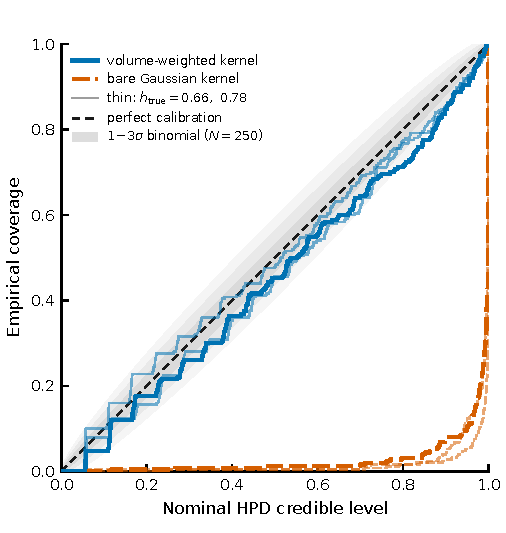
\includegraphics[width=\columnwidth]{figures/fig_pp_coverage.pdf}
  \caption{Probability--probability calibration of the single-host dark-siren posterior on synthetic universes: empirical versus nominal HPD credible level for the bare-Gaussian and volume-deconvolved host-redshift kernels.
  Curves are empirical cumulative distributions of posterior quantiles over 250 realizations of 250 events each, per injected truth $h_{\mathrm{true}} \in \{0.66, 0.72, 0.78\}$ and kernel, computed with the committed harness (\texttt{master\_thesis\_code.validation.pp\_coverage}; $\sigma_z = 0.035$, 5 per cent fractional distance error, $h$-grid step $0.001$; master seed 20260701 with per-realization seeds shared between kernels for an exactly paired comparison). The shaded region is the pointwise binomial acceptance band. The bare-Gaussian kernel (dashed) collapses far below the band (empirical coverage $0.4$--$7$ per cent across all nominal levels); the volume-deconvolved kernel (solid) tracks the diagonal with mild residual under-coverage ($\approx 85$ per cent empirical at the 90 per cent level), consistent with the $\approx -0.002$ residual bias discussed in the text. % src: paper_a/figures/data/fig_pp_coverage_data.json
  }
  \label{fig:pp}
\end{figure}

\subsection{Persistence inside the full completion machinery}
\label{sec:coverage:full}

The clean test isolates the kernel; a companion experiment in the same synthetic framework adds an incomplete catalogue $f(z)$, interloper galaxies with sky-localization weights, the out-of-catalogue completion term, and the selection normalizations $D(h)$ and $\beta_G(h)$ of Section~\ref{sec:framework}. The identical numerator-prior bias survives all of it: at $h_{\mathrm{true}} = 0.72$ the production-style bare-Gaussian numerator peaks at $0.682$ where the volume-deconvolved variant peaks at $0.707$, and the bare variant sits $-0.024$ below it at every injected truth; fixing only the kernel recovers the coverage from $0.00/0.00/0.02$ to $0.40/0.54/0.82$ at the three nominal levels. % src: results/commission_20260701/scratch/d2/coverage_results.json (primary.A_prod, primary.B_corr); NOTE_calibration_findings.md (RESULT 3)
Two residual features of this fuller test --- a $-0.013$ low bias of the corrected estimator and a compressed MAP-versus-truth slope of $\approx 0.35$ shared by \emph{all} non-railing variants --- are traceable to the completion term being only weakly $H_0$-informative when the catalogue is very incomplete, and are sensitive to the synthetic's completeness and interloper modelling; the clean single-host test is therefore the decisive calibration verdict. % src: results/commission_20260701/scratch/d2/NOTE_calibration_findings.md (RESULT 3 discussion)
A diagnostic variant using the literal global selection denominator railed at the grid edge in this synthetic (rail fraction $1.00$); that reflects the delicacy of matching the discrete catalogue number density to $\beta_G$ in a from-scratch mock, not a measurement of the production code, and none of the kernel conclusions depend on it. % src: results/commission_20260701/scratch/d2/coverage_results.json (primary.A_global); NOTE_calibration_findings.md (RESULT 3 caveat)

The harness ships in the code base with the calibrated volume kernel as its default, a command-line interface over the number of realizations and events, $\sigma_z$, the injected truths and the kernel choice, and full determinism: all randomness flows from a single master seed (default $20260701$) through per-realization generators, so every number in this section is exactly reproducible. Its default injected truths ($0.62$, $0.72$, $0.84$) deliberately include near-grid-edge values so that rail behaviour is exercised on every run, and a regression test suite pins the determinism and the volume-beats-bare ordering at $\sigma_z = 0.035$. % src: master_thesis_code/validation/pp_coverage.py (PPCoverageConfig defaults, main); master_thesis_code_test/validation/test_pp_coverage.py
